\newpage

\pagestyle{fancy}
\lhead{\textsc{Chapter 3. CONCEPTION ET RÉALISATION TECHNIQUE}}
\renewcommand{\headrulewidth}{0.5pt}
\renewcommand{\footrulewidth}{0.5pt}

\chapter{CONCEPTION ET RÉALISATION TECHNIQUE}\setlength{\headheight}{28pt}
\label{ch3}
\minitoc

\newpage

\section{Introduction}
Ce chapitre détaille l'implémentation technique du système décisionnel BIOSPHERE. Conformément à la méthodologie Agile adoptée au chapitre précédent, le développement a été structuré en sprints majeurs correspondant aux modules métier : Ventes, Achats, Stock, et Application décisionnelle. Chaque itération suit une chaîne de valeur reproductible : extraction et préparation des données (ETL), alimentation du Data Warehouse (DWH), modélisation analytique (BI/DAX), sécurisation des accès (RLS) et, pour les sprints avancés, intégration du pipeline de Data Science et de l'interface applicative. Cette approche garantit la traçabilité, la robustesse technique et l'alignement strict entre les besoins métier et les livrables développés.
\section{ Section 1: Modélisation et conception des données}
\subsection{Modèle conceptuel de données (MCD)}
Le Modèle Conceptuel de Données est une étape importante entre l'analyse des besoins métier et la modélisation physique du Data Warehouse. Il a pour but de représenter les entités fondamentales du système décisionnel BIOSPHERE de manière abstraite et normalisée, sans tenir compte des technologies. Le Modèle Conceptuel de Données représente également les relations sémantiques qui relient ces entités. Ce modèle sert de référence pour les équipes métier et techniques, et il garantit que la conception analytique reste fidèle aux processus opérationnels de l'entreprise.
\subsubsection{Identification des entités métier}
Et après avoir analysé les flux transactionnels et les besoins décisionnels, sept entités métier centrales ont été identifiées
%================= TABLEAU ENTITÉS =================

{\small
\renewcommand{\arraystretch}{1.2}
\setlength{\tabcolsep}{4pt}


\begin{longtable}{|p{3cm}|p{5cm}|p{9cm}|}

\caption{Dictionnaire des entités métier} \\

\hline
\multicolumn{1}{|c|}{\textbf{Entité}} & 
\multicolumn{1}{c|}{\textbf{Description}} & 
\multicolumn{1}{c|}{\textbf{Attributs clés}} \\ 
\hline
\endfirsthead

\hline
\textbf{Entité} & \textbf{Description} & \textbf{Attributs clés} \\
\hline
\endhead

\hline
\endfoot

Produit & Référence article du catalogue BIOSPHERE & Code\_Article, Désignation, Famille, Sous-famille, PUHT \\
\hline

Client & Tiers de type client (établissements de santé, laboratoires, professionnels) & Code\_Tiers, Nom, Adresse, Ville, Pays, Type \\
\hline

Fournisseur & Tiers de type fournisseur (partenaires d'approvisionnement) & Code\_Tiers, Nom, Conditions d'achat, Délai livraison \\
\hline

Document & En-tête de transaction commerciale (vente, achat, retour) & Doc\_Num, Date\_Doc, Type\_Doc, Site, Doc\_Total, Statut \\
\hline

Ligne\_Document & Détail d'une transaction (produit, quantité, prix) & Quantité, PUHT, MontantHT, TVA, Remise \\
\hline

Mouvement\_Stock & Journal des flux logistiques (entrées, sorties, transferts) & Date\_Mvt, Type\_Mvt, Quantité\_signée, Référence\_doc \\
\hline

Site & Localisation géographique opérationnelle & Code\_Site (TN/SFX), Adresse, Responsable \\
\hline

\end{longtable}

}
\subsubsection{Définition des relations et cardinalités}
Les relations entre entités reflètent la logique métier de BIOSPHERE :

- Un Client passe plusieurs Documents de vente (1,N) ; un Document concerne un seul Client (N,1).

- Un Document contient plusieurs Lignes\_Document (1,N) ; une Ligne\_Document concerne un seul Produit (N,1).

- Un Produit fait l'objet de plusieurs Mouvements\_Stock (1,N) ; un Mouvement\_Stock concerne un seul Produit (N,1).

- Un Document est rattaché à un seul Site (N,1) ; un Site gère plusieurs Documents (1,N).

- Un Fournisseur alimente plusieurs Documents d'achat (1,N) ; un Document d'achat concerne un seul Fournisseur (N,1).
\begin{figure}[H]
    \centering
    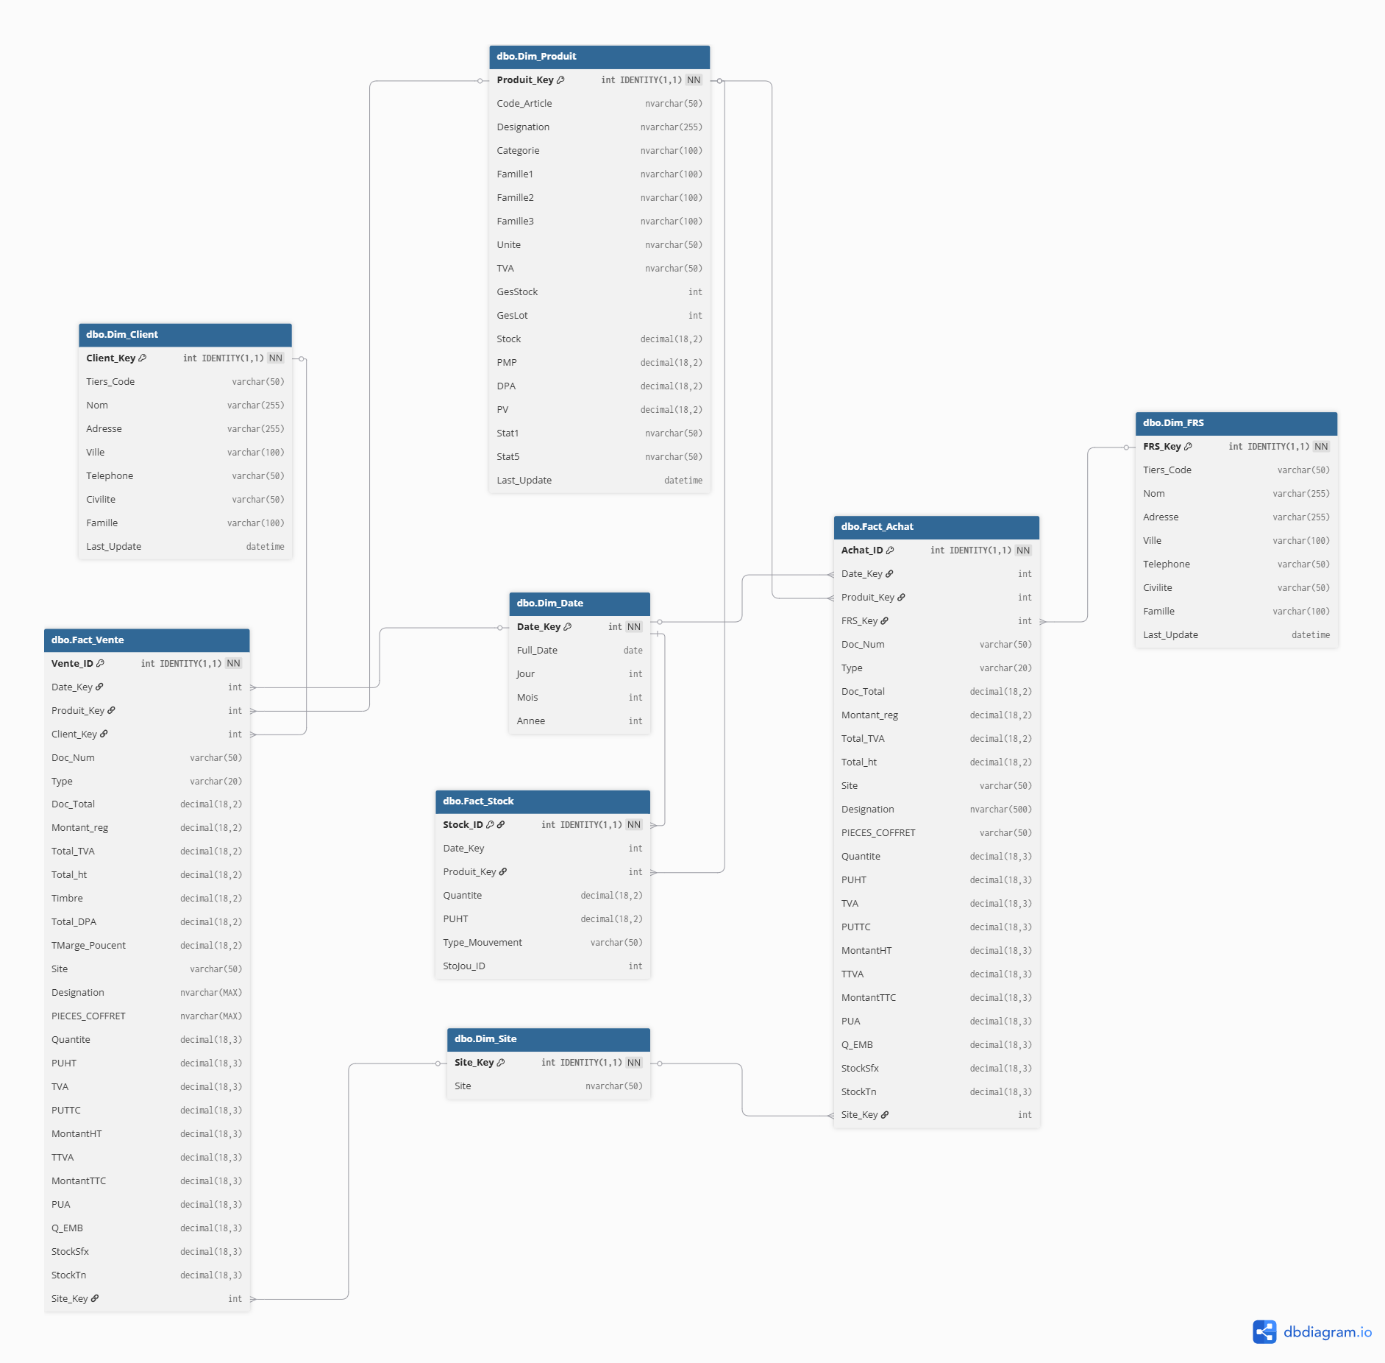
\includegraphics[width=1.1\linewidth]{Figures/Chapitre3/mcd.png}
    \caption{Modèle Conceptuel de Données (MCD) du système décisionnel BIOSPHERE}
    \label{fig:MCD}
\end{figure}
Les entités sont représentées par des rectangles, les relations par des losanges, et les cardinalités indiquent les contraintes d'association. Ce modèle sert de base à la modélisation physique du Data Warehouse en schéma Galaxy.
\subsection{Modèle logique de données }
Passant désormais au modèle logique de données, la transformation du schéma en galaxie a conduit à la mise en place d’une architecture multidimensionnelle composée de tables de dimensions, de tables de faits ainsi que d’une couche de staging dédiée aux traitements ETL. 
Cette modélisation a été conçue dans le but d’optimiser l’exploitation analytique des données liées aux ventes, aux achats et à la gestion des stocks, tout en garantissant la cohérence, la performance et la traçabilité des informations décisionnelles.\\
Il se rédige de la façon suivante : 
\begin{itemize}
    \item \textbf{Dim\_Produit} (Code\_Produit\#, Produit\_Key, Designation, Famille1, Famille2, PUHT, Date\_Creation, Last\_Update)
    \item \textbf{Dim\_Client} (Code\_Tiers\#, Client\_Key, Nom\_Client, Adresse, Ville, Pays, Type, Date\_Creation, Last\_Update)
    \item \textbf{Dim\_FRS }(Code\_Tiers\#, FRS\_Key, Nom\_Fournisseur, Adresse, Ville, Pays, Type, Conditions\_Paiement, Date\_Creation, Last\_Update)
    \item \textbf{Dim\_Date} (Date\_Key\#, Full\_Date, Jour, Mois, Annee, Trimestre, Semaine, DayOfWeek, IsWeekend)
    \item \textbf{Dim\_Site} (Site\_Code\#, Site\_Key, Nom\_Site, Adresse, Responsable, Region)
    \item \textbf{Fact\_Vente} (Vente\_ID\#, Date\_Key\#, Produit\_Key\#, Client\_Key\#, Site\_Key\#, Doc\_Num, Type\_Doc, Doc\_Total, Montant\_reg, Total\_TVA, Total\_ht, Timbre, Total\_DPA, TMarge\_Poucent, Site, Designation, Quantite, PUHT, MontantHT, MontantTTC, StockSfx, StockTn, Date\_Chargement)
    \item \textbf{Fact\_Achat} (Achat\_ID\#, Date\_Key\#, Produit\_Key\#, FRS\_Key\#, Site\_Key\#, Doc\_Num, Type\_Doc, Doc\_Total, Montant\_reg, Total\_TVA, Total\_ht, Site, Designation, Quantite, PUHT, MontantHT, MontantTTC, StockSfx, StockTn, Date\_Chargement)
    \item \textbf{Fact\_Stock} (Stock\_ID\#, Date\_Key\#, Produit\_Key\#, Quantite, PUHT, Type\_Mouvement, StoJou\_ID, Signe\_Mouvement, Date\_Chargement)
    \item \textbf{STG\_DOCUMENT} (Doc\_ID\#, Doc\_Num, Type\_Doc, Code\_Tiers, Date\_Doc, Doc\_Total, Site, Code\_Article, Quantite, PUHT, MontantHT, Last\_Extract)
    \item \textbf{STG\_ARTICLE} (Article\_ID\#, Code\_Article, Designation, Famille1, Famille2, PUHT, Actif, Last\_Extract)
    \item \textbf{STG\_TIERS }(Tiers\_ID\#, Code\_Tiers, Nom, Adresse, Ville, Pays, Type, Last\_Extract)
    \item \textbf{STG\_STOJOU} (StoJou\_ID\#, Code\_Article, Date\_Mvt, Type\_Mvt, Quantite, Signe, Doc\_Ref, Last\_Extract)
    \item \textbf{STG\_CTRL\_CHARGEMENT} (Table\_Name\#, Last\_Timestamp, Record\_Count, Status, Last\_Update)
\end{itemize}
\subsection{Architecture technique}
\subsubsection{Conteneurisation avec Docker}
L’environnement technique du projet repose sur une architecture conteneurisée basée sur Docker, adoptée afin d’assurer l’isolation des services, la portabilité de la solution ainsi qu’une meilleure stabilité des traitements. Dans ce cadre, l’outil d’orchestration n8n a été déployé dans un conteneur dédié à partir de l’image officielle n8nio/n8n. L’interface web de gestion des workflows est exposée via le port 5678, permettant ainsi l’administration et le suivi des processus ETL (Figure 21). Cette approche facilite également le déploiement et réduit les dépendances liées à l’environnement local de développement.
\begin{figure}[H]
    \centering
    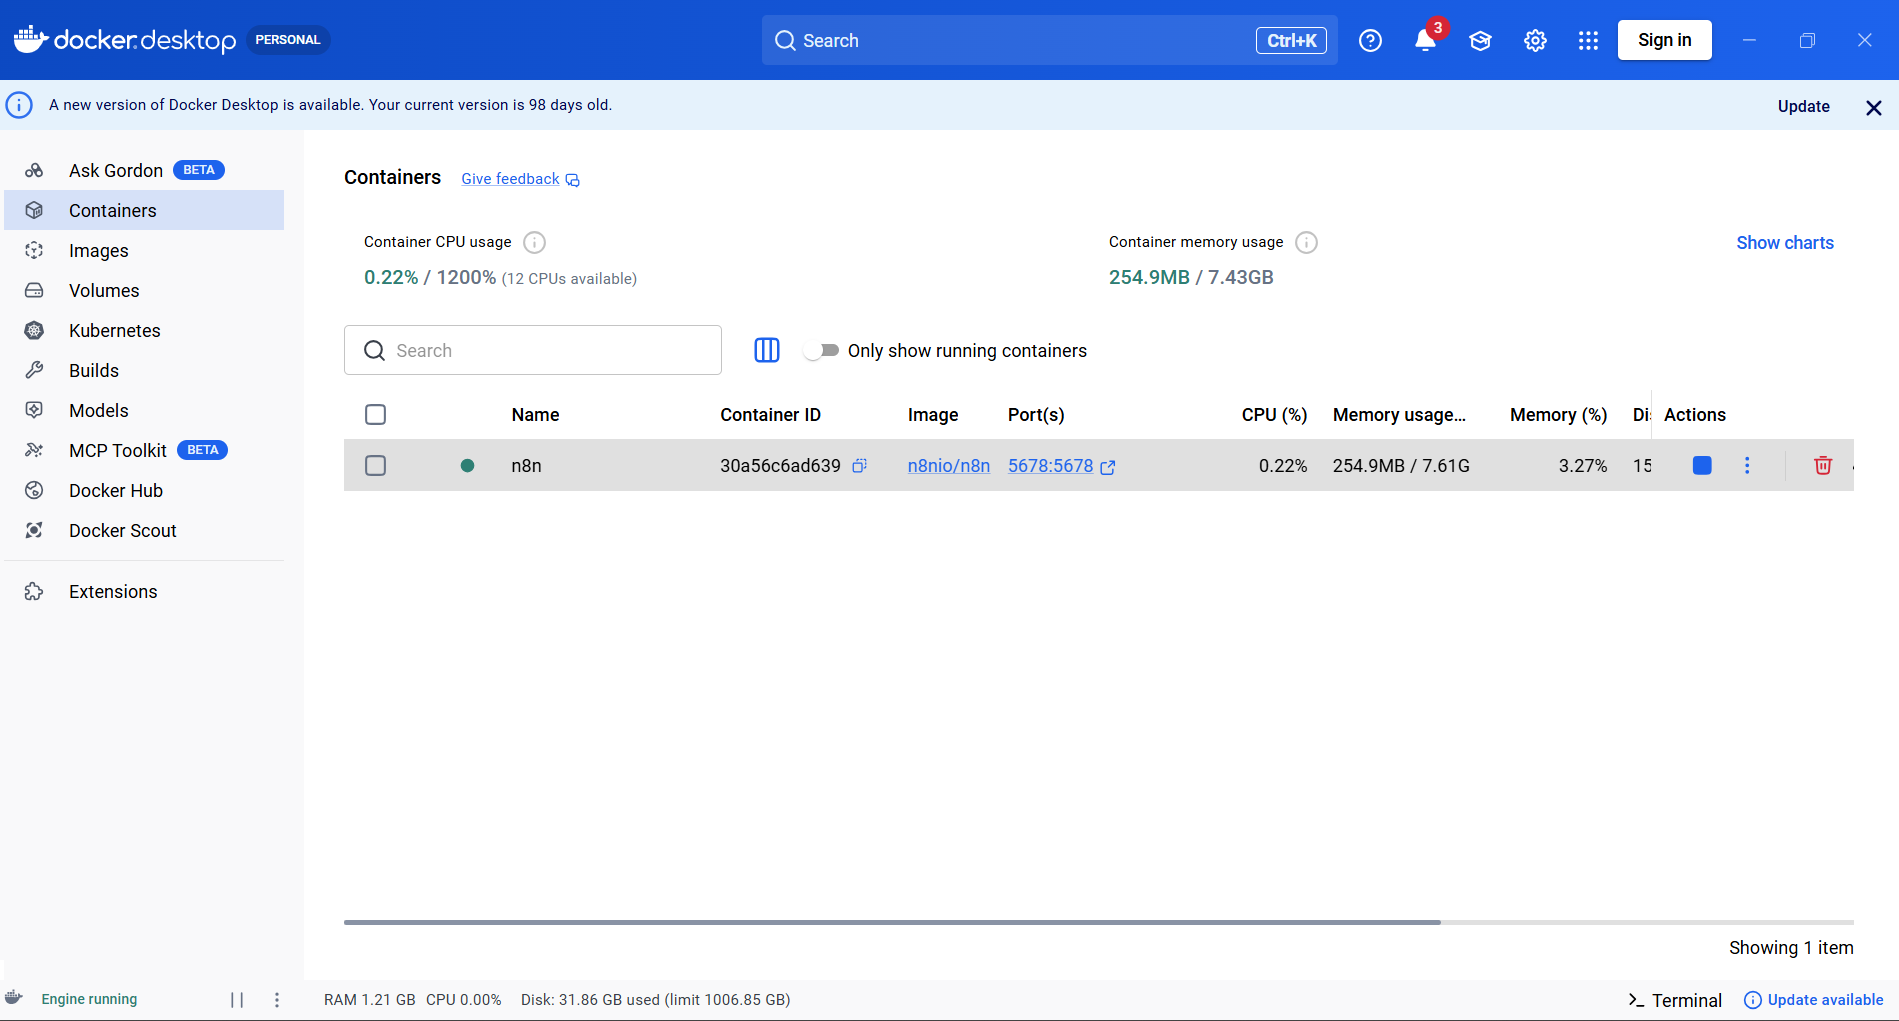
\includegraphics[width=1.1\linewidth]{Figures/Chapitre3/docker.png}
    \caption{Conteneur Docker n8n en cours d’exécution}
    \label{fig:docker}
\end{figure}
\subsubsection{Orchestration des workflows ETL avec n8n}
Le processus ETL mis en place repose sur une architecture en deux niveaux garantissant la qualité, la cohérence et la traçabilité des données. Dans une première étape, les données sont extraites depuis la base opérationnelle BIOSPHERE puis chargées dans une couche de staging nommée ERP\_STG. Cette couche intermédiaire joue le rôle d’une zone tampon dédiée au nettoyage, à la transformation et à la normalisation des données. Elle permet également d’assurer une meilleure sécurité du processus ETL en limitant les risques de perte de données ou de corruption en cas de panne, d’erreur de chargement ou de crash du système. Grâce à cette séparation entre les données sources et le Data Warehouse final, les traitements peuvent être rejoués et contrôlés plus facilement, garantissant ainsi la fiabilité et l’intégrité des données décisionnelles.\\
Dans une seconde étape, les données préparées sont transférées vers le Data Warehouse analytique ERP\_DWH, où elles sont organisées selon une modélisation en galaxie afin d’optimiser les traitements analytiques et décisionnels.\\
Afin d’assurer une mise à jour régulière Cela nous permet de calculer et d'afficher des données sans perturber les opérations métier, les workflows ETL ont été configurés pour s’exécuter automatiquement chaque jour à 04:00 du matin (Figure 22), correspondant à une période de faible activité transactionnelle. 
\begin{figure}[H]
    \centering
    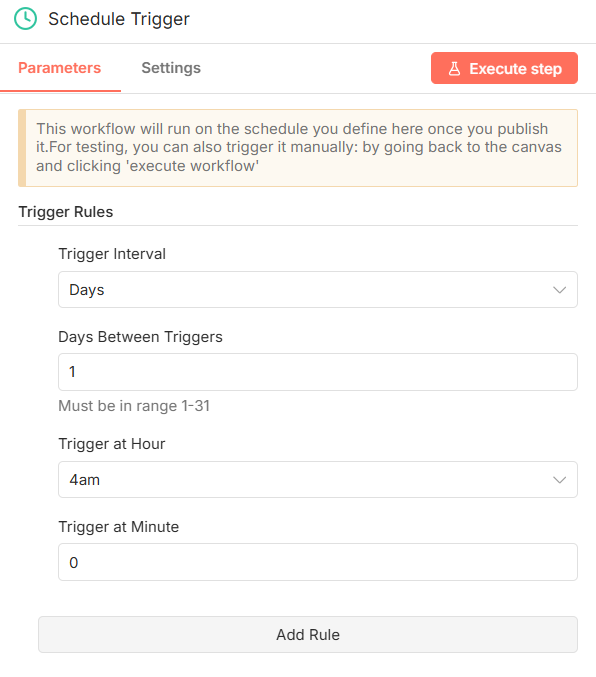
\includegraphics[width=0.5\linewidth]{Figures/Chapitre3/timer.png}
    \caption{heure du lancement du workflow du STG}
    \label{fig:timer}
\end{figure}
Cette planification permet de garantir une synchronisation quotidienne entre la couche de staging et le Data Warehouse. En complément, le système conserve également la possibilité d’un déclenchement manuel des workflows.\\
L’architecture mise en place repose sur deux workflows distincts mais dépendant entre eux afin de renforcer la modularité et la traçabilité du processus ETL. Le premier workflow est dédié à l’alimentation de la couche de staging (Figure 22), tandis que le second assure le chargement des données transformées vers le Data Warehouse final (Figure 23). Cette séparation permet d’améliorer la robustesse, la maintenabilité et le suivi des opérations de mise à jour des données décisionnelles.
\begin{figure}[H]
    \centering
    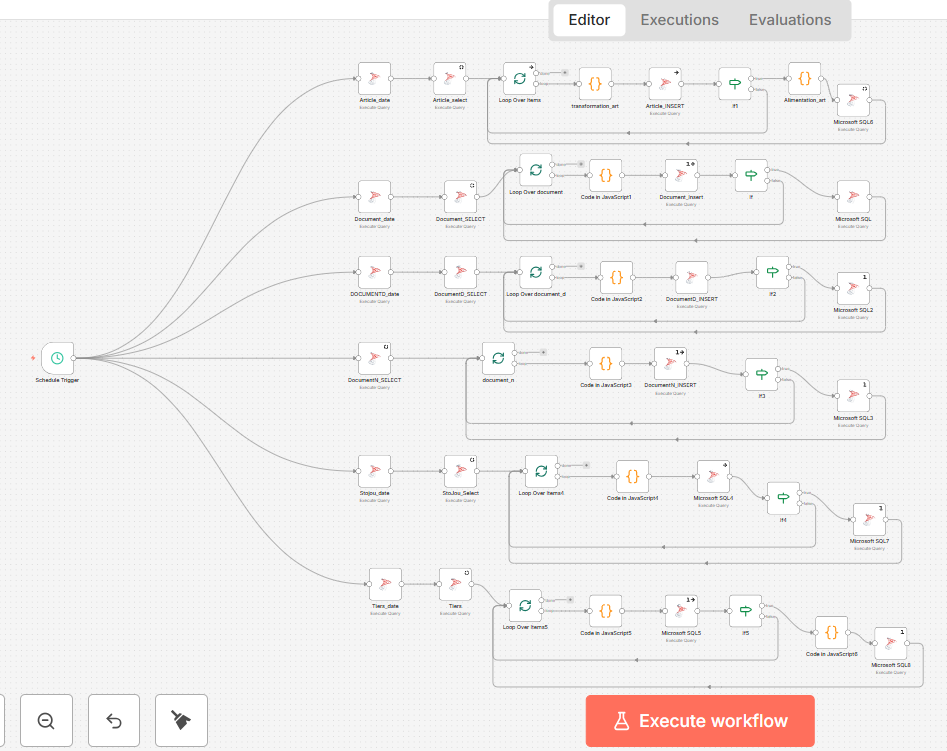
\includegraphics[width=1.1\linewidth]{Figures/Chapitre3/workflow_bd.png}
    \caption{workflow alimentation de BD staging }
    \label{fig:workflowBD}
\end{figure}
\begin{figure}[H]
    \centering
    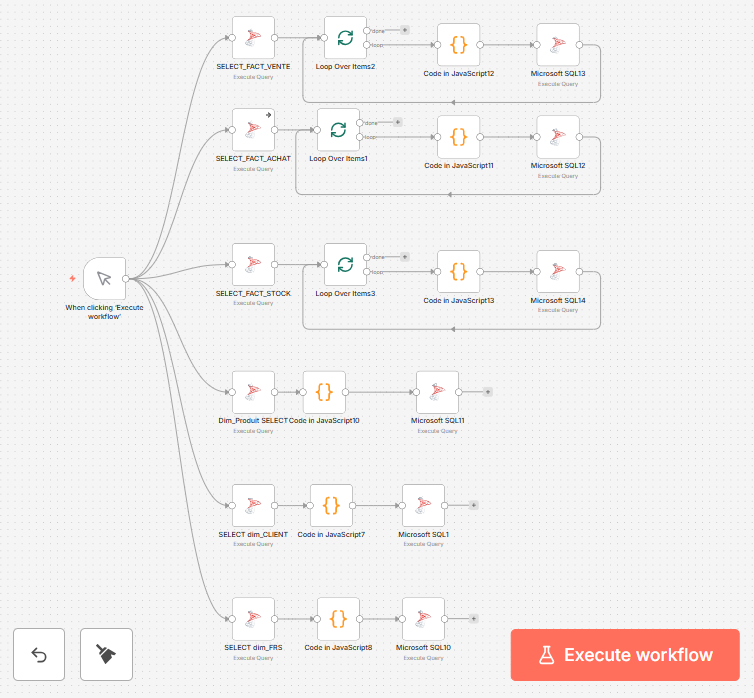
\includegraphics[width=0.9\linewidth]{Figures/Chapitre3/workflow_dwh.png}
    \caption{workflow alimentation de la DWH}
    \label{fig:workflowDWH}
\end{figure}
\subsection{Configuration de la base de données }               
Les bases opérationnelles, la couche de staging (ERP\_STG) et le Data Warehouse (ERP\_DWH) résident sur une instance Microsoft SQL Server (SHAIMA/SQLSRV). La configuration réseau a été validée via l'activation du protocole TCP/IP, l'écoute sur le port 1433, et le démarrage du service SQL Server Browser. L'authentification repose sur le mode mixte (Windows/SQL), avec un compte technique dédié aux pipelines ETL et aux connexions applicatives. Cette configuration assure une communication stable entre les outils d'orchestration (n8n), les scripts Python et le moteur relationnel.
\begin{figure}[H]
    \centering
    
\includegraphics[width=0.8\linewidth]{Figures/Chapitre3/login.png}
    \caption{Configuration de la base de données}
    \label{fig:login}
\end{figure}
\subsection{Implémentation du Row-Level Security (RLS) dans POWER BI}
Afin de garantir la sécurité et la confidentialité des données selon le périmètre de chaque utilisateur, nous avons implémenté un mécanisme de Row-Level Security (RLS) dans Power BI. Trois rôles ont été configurés :
\begin{itemize}
    \item Directeur : accès global à toutes les données (Tunis et Sfax)
    \item Manager\_TN : accès restreint aux données du site de Tunis uniquement
    \item Manager\_SFX : accès restreint aux données du site de Sfax uniquement
\end{itemize}
Cette approche garantit qu'un manager ne peut visualiser que les transactions relatives à son site, tandis que la direction conserve une vision consolidée.\\
La validation du RLS a été effectuée dans Power BI Desktop à l'aide de la fonctionnalité "Afficher comme rôles", confirmant le bon fonctionnement des restrictions d'accès avant publication.
\begin{figure}[H]
    \centering
    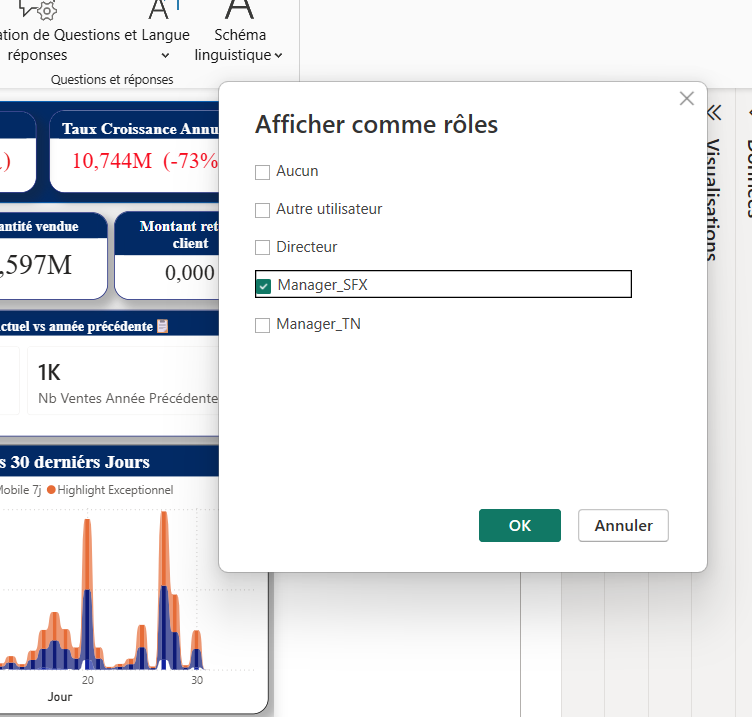
\includegraphics[width=0.7\linewidth]{Figures/Chapitre3/securite.png}
    \caption{Implémentation du Row-Level Security (RLS) dans POWER BI}
    \label{fig:sécurité}
\end{figure}
\section{Section 2 : la réalisation des sprints }
\subsection{Sprint 1 : Module Ventes}
\subsubsection{Objectifs du sprint}
Dans le cadre du développement du module Business Intelligence pour les ventes, nous avons mis en place une connexion directe avec le Data Warehouse ERP\_DWH. Cela nous permet de calculer et d'afficher les principaux indicateurs clés de performance commerciale à partir d'une connexion SQL Server.\\
Le système que nous avons développé permet également d'appliquer un mécanisme de filtrage basé sur les rôles des utilisateurs. Nous utilisons le principe du Row-Level Security pour offrir un accès différencié en fonction du profil connecté. 
%================= TABLE SPRINT 1 =================

{ \small
\renewcommand{\arraystretch}{1.2} % Un stretch de 1.5 suffit souvent et évite les tableaux trop géants
\setlength{\tabcolsep}{4pt}

% Somme des colonnes réduite pour tenir dans les marges (Ex: 2.5 + 2.5 + 1.2 + 1.5 + 4.5 = 12.2cm)
\begin{longtable}{|p{3cm}|p{2.5cm}|p{1.2cm}|p{2cm}|p{4.5cm}|}
\caption{Sprint 1 : Module Vente} \\
\hline
\multicolumn{1}{|c|}{\textbf{Sprint / Phase}} & 
\multicolumn{1}{c|}{\textbf{User Stories concernées}} & 
\multicolumn{1}{c|}{\textbf{Priorité}} & 
\multicolumn{1}{c|}{\textbf{Durée estimée}} & 
\multicolumn{1}{c|}{\textbf{Livrable attendu}} \\
\hline
\endfirsthead

\hline

\textbf{Sprint / Phase} & \textbf{User Stories concernées} & \textbf{Priorité} & \textbf{Durée estimée} & \textbf{Livrable attendu} \\
\hline
\endhead

\hline
\endfoot

Sprint 1 : Module Vente & US07, US03, US02, US01 & Haute & 2 semaines & Dashboard ventes, KPI commerciaux, analyse des tendances des ventes \\
\hline

\end{longtable}

}
\subsubsection{Les KPIs de vente}
%================= TABLE KPIs VENTE =================

{\small
\renewcommand{\arraystretch}{1.2}
\setlength{\tabcolsep}{4pt}


\begin{longtable}{|p{3.5cm}|p{3.2cm}|p{5cm}|p{5cm}|}

\caption{Les KPIs de vente} \\

\hline
\multicolumn{1}{|c|}{\textbf{Catégorie}} & 
\multicolumn{1}{c|}{\textbf{KPI}} & 
\multicolumn{1}{c|}{\textbf{Formule de calcul}} & 
\multicolumn{1}{c|}{\textbf{Source de données}} \\
\hline
\endfirsthead

\hline
\rowcolor{cyan!10}
\textbf{Catégorie} & \textbf{KPI} & \textbf{Formule de calcul} & \textbf{Source de données} \\
\hline
\endhead

\hline
\endfoot

Performance commerciale & Chiffre d'affaires total & SUM(Fact\_Vente.Doc\_Total) & Fact\_Vente + Dim\_Date \\
\hline

Rentabilité & Marge brute & [Ventes] - [Achats] & Fact\_Vente + Fact\_Achat \\
\hline

Rentabilité & Taux de marge (\%) & DIVIDE([Marge], [Ventes]) * 100 & Fact\_Vente + Fact\_Achat \\
\hline

Performance & Profit net & [Ventes] - [Achats] & Fact\_Vente + Fact\_Achat \\
\hline

Analyse temporelle & Évolution CA vs N-1 & ([CA\_N] - [CA\_N-1]) / [CA\_N-1] * 100 & Fact\_Vente + Dim\_Date \\
\hline

Produits & Top 10 produits par CA & TOPN (10, Produits, [CA]) & Fact\_Vente + Dim\_Produit \\
\hline

Performance & Panier moyen & [CA Total] / [Nombre de ventes] & Fact\_Vente \\
\hline

Objectifs & Taux de réalisation objectif CA & [CA Réalisé] / [Objectif CA] * 100 & Fact\_Vente + Objectifs \\
\hline

\end{longtable}

}
\subsubsection{Réalisation technique }
Dans cette section, nous présentons de manière détaillée le workflow d'alimentation de la table STG.ARTICLE à titre d'exemple illustratif. Il inclue l'extraction depuis la base source, les transformations JavaScript nécessaires au nettoyage et à la normalisation des données, ainsi que le chargement incrémental dans la couche de staging. Les workflows relatifs aux autres tables (DOCUMENT, DOCUMENT\_D, TIERS, STOJOU) suivent une logique similaire et sont présentés en annexe. \\

\textbf{a)	Exemple du workflow de la table articles}
\begin{figure}[H]
    \centering
    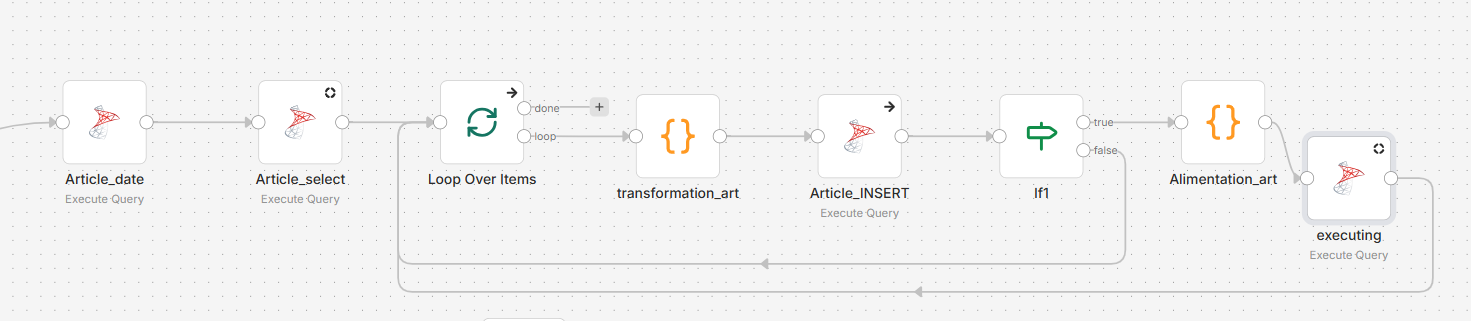
\includegraphics[width=0.99\linewidth]{Figures/Chapitre3/workflow_art.png}
    \caption{workflow ETL article}
    \label{fig:WORKFLOW ART}
\end{figure}

\textbf{b)	Extraction depuis la base BIOSPHERE}
\begin{itemize}
    \item Tables sources extraites :
\end{itemize}
Le processus d'extraction et d'analyse des données repose sur plusieurs tables clés issues de la base de données source biosphere. Les en-têtes et les détails des transactions commerciales sont récupérés via les tables dbo.Document (en-têtes de documents de vente) et dbo.DocumentD (lignes de documents). Le référentiel métier est quant à lui enrichi par les tables dbo.Art, qui liste l'ensemble des articles et produits, et dbo.Tiers, qui centralise les informations relatives aux clients et fournisseurs. Enfin, la table dbo.StoJou, dédiée aux mouvements de stock.
\begin{figure}[H]
    \centering
    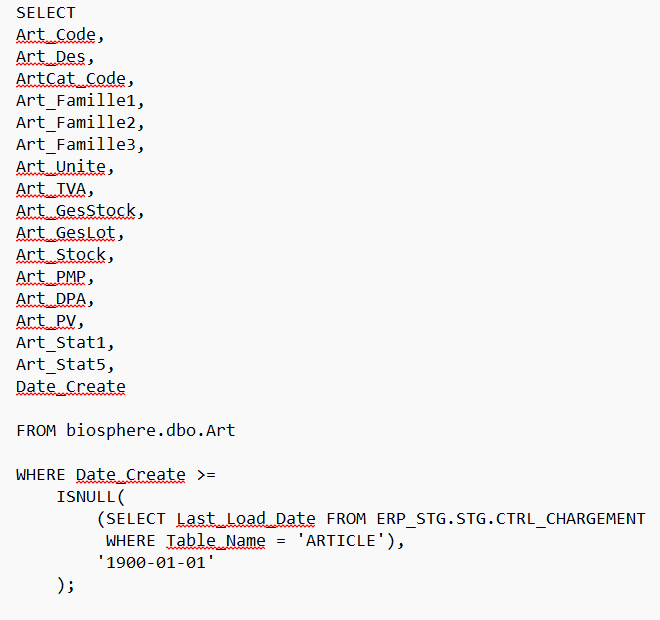
\includegraphics[width=0.7\linewidth]{Figures/Chapitre3/requete_art.png}
    \caption{Exemple d’une requête d’Extraction des articles depuis la base BIOSPHERE}
    \label{fig:REQUETEART}
\end{figure}

\textbf{c)	Alimentation de ERP\_STG par workflow n8n}
\begin{itemize}
    \item Tables de staging alimentées :
\end{itemize}
L'alimentation des tables de la couche de staging (ERP\_STG) repose sur un traitement rigoureux des données à l'aide de scripts JavaScript. Ce code intervient en amont pour réaliser les jointures nécessaires entre les tables sources et nettoyer les données en supprimant les doublons résiduels. Ce processus permet de charger de manière optimale les cinq tables cibles suivantes :
\begin{itemize}
    \item STG.DOCUMENT : Centralisation de tous les types de documents de vente.
    \item STG.DOCUMENT\_D : Détails et lignes des documents.
    \item STG.ARTICLE : Référentiel des produits normalisés.
    \item STG.TIERS : Fiches centralisées des clients et fournisseurs.
    \item STG.CTRL\_CHARGEMENT : Table technique dédiée au suivi incrémental.
\end{itemize}
\begin{figure}[H]
    \centering
    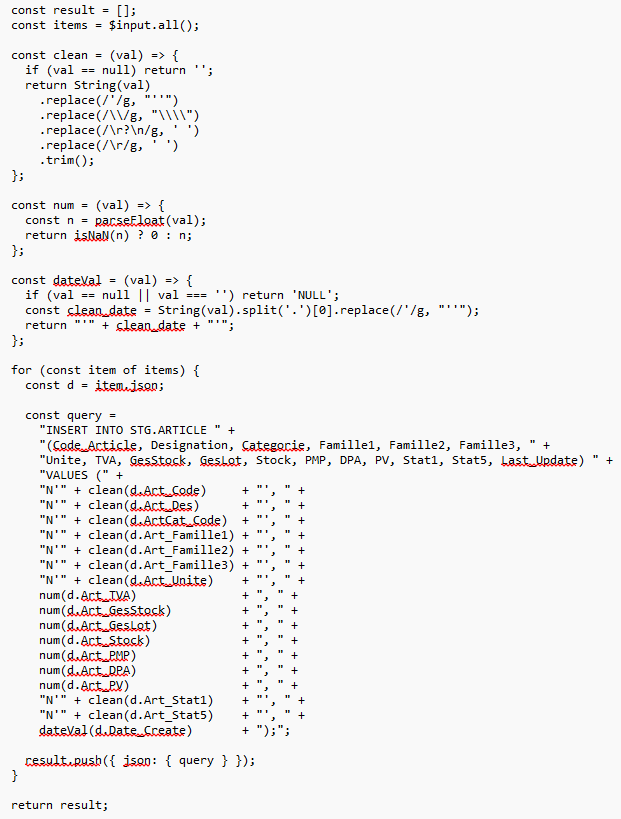
\includegraphics[width=0.9\linewidth]{Figures/Chapitre3/code_js_article.png}
    \caption{Exemple du code JS pour insertion de la table stg.Article}
    \label{fig:code JS}
\end{figure}
La phase d'intégration s'appuie sur une logique stricte de chargement incrémental. En utilisant la table STG.CTRL\_CHARGEMENT, le système tracke le dernier timestamp d'exécution afin de réaliser une extraction différentielle, limitant le flux aux seules lignes créées ou modifiées depuis le dernier traitement. Enfin, l'application finale des données en base utilise des commandes MERGE, garantissant une mise à jour fluide et une protection absolue contre l'apparition de doublons\\

\textbf{d)	Alimentation de ERP\_DWH}\\
L'alimentation de la couche décisionnelle ERP\_DWH par le workflow suivant :
Elle s'appuie sur une modélisation en Galaxy, composée de quatre dimensions et d'une table de faits centrale. Le référentiel des dimensions est constitué de :
\begin{itemize}
    \item Dim\_Date : Comprend 4 383 lignes, structurées autour de la clé primaire Date\_Key.
    \item Dim\_Produit : Alimentée directement depuis STG.ARTICLE, elle regroupe 4 952 lignes identifiées par la clé Produit\_Key.
    \item Dim\_Client : Contient 3 120 lignes basées sur la clé Client\_Key, après l'application d'un filtre strict sur le type de tiers (Type='01').
    \item Dim\_Site : Une dimension de 2 lignes distinguant les sites géographiques (TN et SFX).
\end{itemize}
La table de faits centrale, Fact\_Vente, totalise quant à elle 260 227 lignes. Sa construction repose sur une jointure initiale d'enrichissement entre les tables de staging STG.DOCUMENT et STG.DOCUMENT\_D. Pour finaliser la structure de Galaxy et assurer la traçabilité des indicateurs, des jointures successives (LEFT/INNER JOIN) sont appliquées avec les dimensions clés : Dim\_Date (via Date\_Key), Dim\_Produit (via Produit\_Key), et Dim\_Client (via Client\_Key).
\begin{figure}[H]
    \centering
    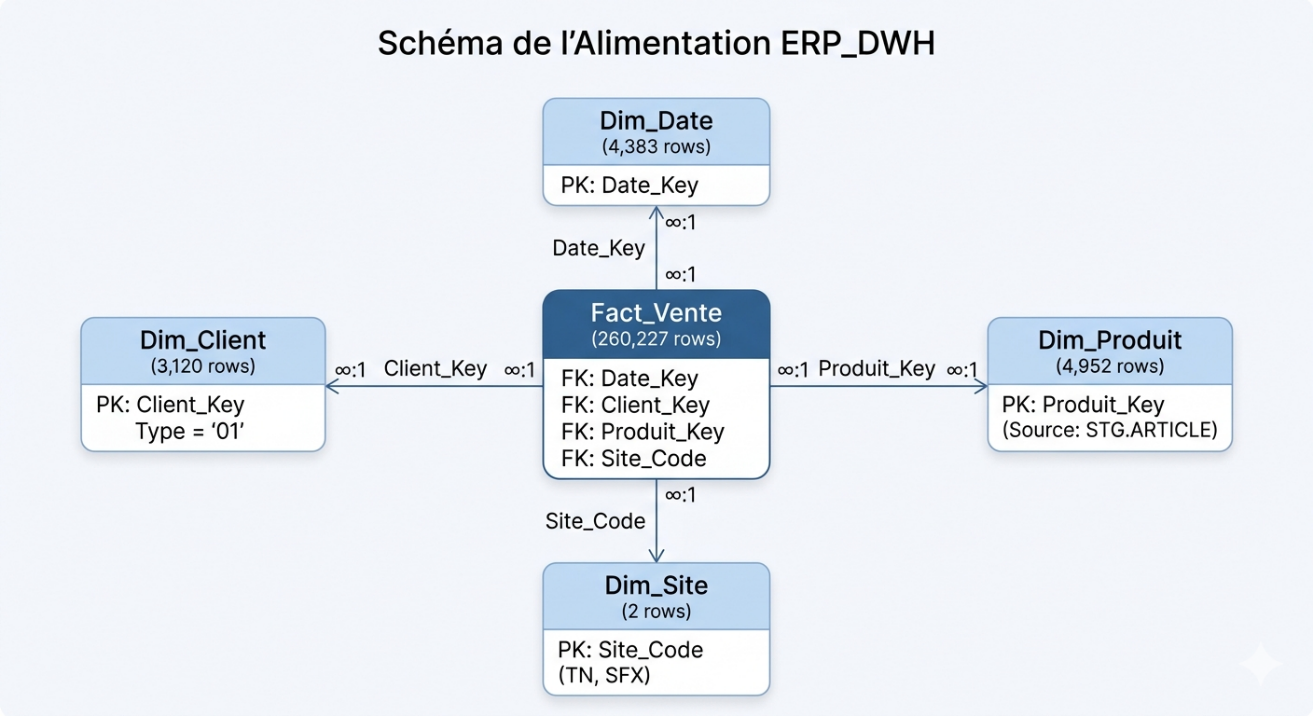
\includegraphics[width=0.9\linewidth]{Figures/Chapitre3/modele_conceptuel_vente.png}
    \caption{modèle conceptuel « Fact\_Vente »}
    \label{fig:modéleC}
\end{figure}

\textbf{e)	Dashboarding }
\begin{itemize}
    \item \textbf{Connexion avec Power BI} 
\end{itemize}
\textbf{•	Configuration de la source }\\
o	Type : SQL Server\\
o	Serveur : SHAIMA/SQLSRV\\
o	Base : ERP\_DWH\\
o	Authentification : Windows / SQL Server
\begin{itemize}
    \item \textbf{Préparation des DAX} 
\end{itemize}
\begin{figure}[H]
    \centering
    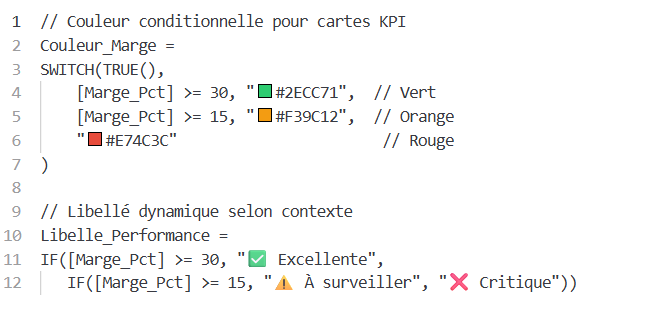
\includegraphics[width=0.7\linewidth]{Figures/Chapitre3/exemple_dax.png}
    \caption{exemple des DAX pour le dashboard performance Globale}
    \label{fig:exempledax}
\end{figure}
\begin{itemize}
    \item \textbf{Visuels implémentés}
\end{itemize}
\begin{figure}[H]
    \centering
    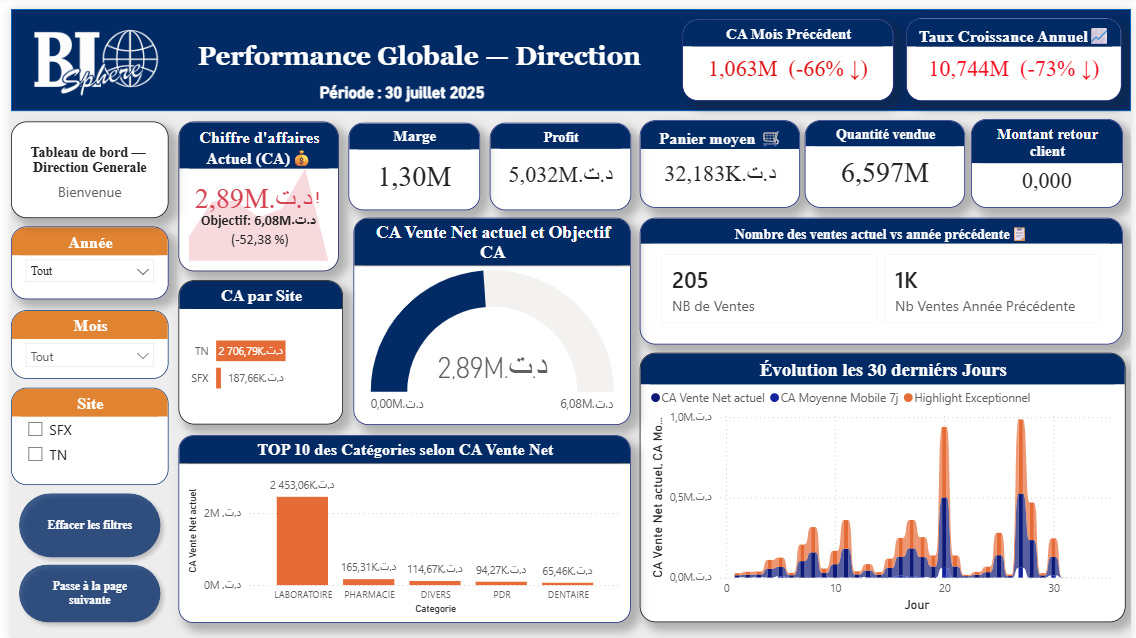
\includegraphics[width=0.9\linewidth]{Figures/Chapitre3/dashboard_vente_1.png}
    \caption{Dashboard-vente :  Page performance Globale}
    \label{fig:dashboardvente}
\end{figure}
\begin{figure}[H]
    \centering
    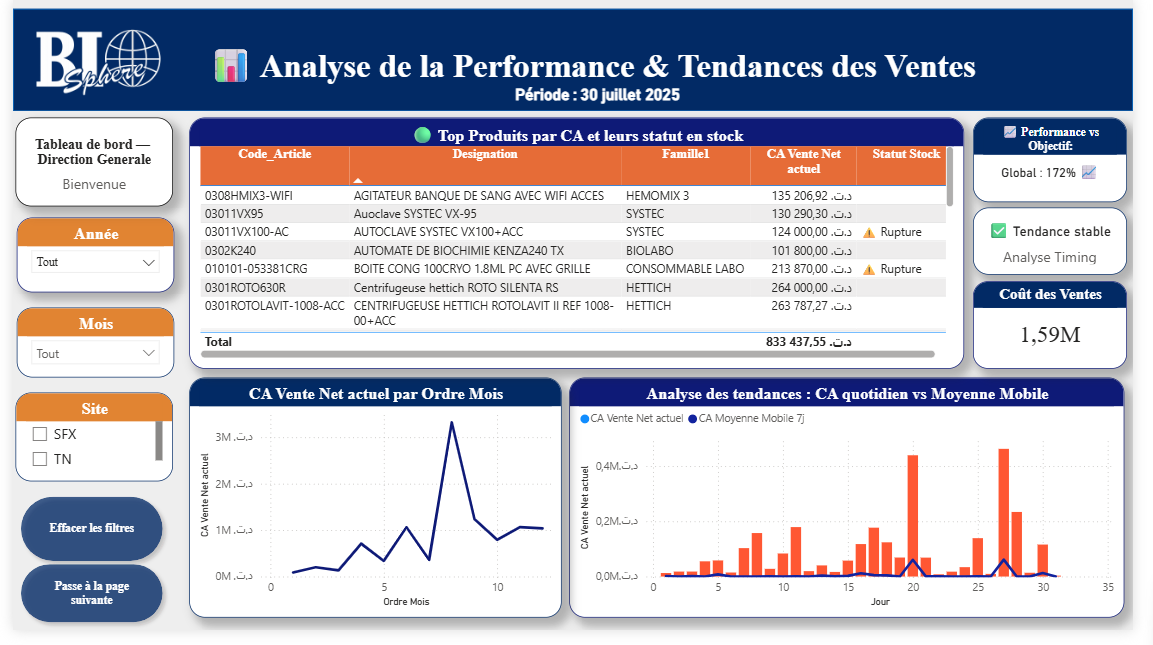
\includegraphics[width=0.9\linewidth]{Figures/Chapitre3/dashboard_vente_2.png}
    \caption{Dashboard-vente :  page Analyse de la performance \& tendances des ventes}
    \label{fig:dashboardvente2}
\end{figure}
\subsubsection{Interprétation globale du module ventes}
%================= TABLE INTERPRÉTATION MODULE VENTES =================

{\small
\renewcommand{\arraystretch}{1.2}
\setlength{\tabcolsep}{4pt}

\begin{longtable}{|p{5cm}|p{5cm}|p{6.5cm}|}

\caption{Interprétation globale du module ventes} \\

\hline
\multicolumn{1}{|c|}{\textbf{Points forts}} & 
\multicolumn{1}{c|}{\textbf{Points critiques}} & 
\multicolumn{1}{c|}{\textbf{Actions prioritaires}} \\
\hline
\endfirsthead

\hline
\multicolumn{1}{|c|}{\textbf{Points forts}} & 
\multicolumn{1}{c|}{\textbf{Points critiques}} & 
\multicolumn{1}{c|}{\textbf{Actions prioritaires}} \\
\hline
\endhead

\hline
\endfoot

Profit net positif (5,032M) & CA à -52,38\% de l'objectif & 1. Analyser les causes de la baisse des ventes (-79,5\%) \\
\hline

Performance vs objectif à 172\% & Ruptures de stock multiples & 2. Réapprovisionner les produits en rupture \\
\hline

Tendance stable & Site Sfax sous-performant (187K vs 2,7M) & 3. Renforcer l'activité commerciale à Sfax \\
\hline

Retour client nul & Forte dépendance LABORATOIRE & 4. Diversifier l'offre produits \\
\hline

 & Volatilité des ventes journalières & 5. Mettre en place des actions promotionnelles \\
\hline
\end{longtable}

}
Ce sprint a permis de mettre en place une première couche analytique dédiée au suivi des ventes, garantissant la disponibilité des indicateurs commerciaux en temps réel.
\subsection{Sprint 2 : Module Achats}
Après la mise en œuvre du module ventes, le projet s’est orienté vers l’intégration des flux d’approvisionnement à travers le module achats.
\subsubsection{Objectifs du sprint}
Le deuxième sprint a porté sur la mise en place du module Achats. Ce module a été développé en parallèle avec le Sprint 1. 
Il a permis de réaliser plusieurs étapes importantes. Par exemple, nous avons développé la fonction fetch\_fact\_achat. Cette fonction a amélioré la sécurité de l'extraction des données d'achat qui a permis de calculer avec précision des indicateurs clés tels que le montant total des achats, le nombre de fournisseurs actifs et la fréquence des commandes.
En combinant ces nouvelles données avec celles des ventes, le système peut maintenant calculer automatiquement le profit et la marge brute. La marge brute est calculée en soustrayant les achats des ventes. 
%================= TABLE SPRINT 2 =================

{\small
\renewcommand{\arraystretch}{1.2}
\setlength{\tabcolsep}{4pt}


\begin{longtable}{|p{3cm}|p{2.5cm}|p{1.2cm}|p{2cm}|p{4.5cm}|}

\caption{Sprint 2 : Module Achats} \\

\hline
\multicolumn{1}{|c|}{\textbf{Sprint / Phase}} & 
\multicolumn{1}{c|}{\textbf{User Stories concernées}} & 
\multicolumn{1}{c|}{\textbf{Priorité}} & 
\multicolumn{1}{c|}{\textbf{Durée estimée}} & 
\multicolumn{1}{c|}{\textbf{Livrable attendu}} \\
\hline
\endfirsthead

\hline
\textbf{Sprint / Phase} & \textbf{User Stories concernées} & \textbf{Priorité} & \textbf{Durée estimée} & \textbf{Livrable attendu} \\
\hline
\endhead

\hline
\endfoot

Sprint 2 : Module Achat & US07, US03, US02, US01 & Moyenne & 2 semaines & Dashboard achats, suivi des fournisseurs et indicateurs d'approvisionnement \\
\hline

\end{longtable}

}
\subsubsection{Les KPIs d’achat}
%================= TABLE KPIs ACHAT =================

{\small
\renewcommand{\arraystretch}{1.2}
\setlength{\tabcolsep}{4pt}


\begin{longtable}{|p{2.8cm}|p{2.8cm}|p{4.5cm}|p{4.5cm}|}

\caption{Les KPIs d'achat} \\

\hline
\multicolumn{1}{|c|}{\textbf{Catégorie}} & 
\multicolumn{1}{c|}{\textbf{KPI}} & 
\multicolumn{1}{c|}{\textbf{Formule de calcul}} & 
\multicolumn{1}{c|}{\textbf{Source de données}} \\
\hline
\endfirsthead

\hline
\multicolumn{1}{|c|}{\textbf{Catégorie}} & 
\multicolumn{1}{c|}{\textbf{KPI}} & 
\multicolumn{1}{c|}{\textbf{Formule de calcul}} & 
\multicolumn{1}{c|}{\textbf{Source de données}} \\
\hline
\endhead

\hline
\endfoot

Volume achats & Total Achats & SUM (Fact\_Achat.Doc\_Total) & Fact\_Achat + Dim\_Date \\
\hline

Coûts & Coût moyen pondéré & SUM(MontantHT) / SUM(Quantité) & Fact\_Achat \\
\hline

Fournisseurs & Nombre de fournisseurs actifs & DISTINCTCOUNT (Fact\_Achat[FRS\_Key]) & Fact\_Achat + Dim\_FRS \\
\hline

Performance & Croissance des achats & ([Achats\_N] - [Achats\_N-1]) / [Achats\_N-1] * 100 & Fact\_Achat + Dim\_Date \\
\hline

Rentabilité & Rentabilité par catégorie & [Profit] / [Total Achats] & Fact\_Achat + Fact\_Vente \\
\hline

Approvisi-onnement & Fréquence d'achat par produit & COUNT (Fact\_Achat[Doc\_Num]) & Fact\_Achat + Dim\_Produit \\
\hline

Qualité & Répartition achats par fournisseur & DIVIDE ([Achats FRS], [Total Achats]) * 100 & Fact\_Achat + Dim\_FRS \\
\hline

Prix & Prix moyen d'achat & SUM(MontantHT) / SUM(Quantité) & Fact\_Achat \\
\hline

\end{longtable}
}
\subsubsection{Réalisation technique}

\textbf{a)	Extraction depuis la base BIOSPHERE}\\
Dans le cadre du déploiement du module Achats, la phase d'extraction cible spécifiquement les flux d'approvisionnement depuis la base source BIOSPHERE afin de compléter l'infrastructure existante. Cette étape repose sur la récupération des en-têtes et des lignes de transactions via les tables transactionnelles dbo.Document et dbo.DocumentD, complétées par les données de la table des articles dbo.Art. Pour isoler précisément les flux d'achats, le processus applique dès la source un filtrage strict sur ce type de document ainsi qu'une restriction historique pour collecter les données. Enfin, l'ensemble est enrichi par une jointure avec la table dbo.Tiers, configurée pour ne retenir que les fournisseurs grâce à un filtre sur le type de tiers égal à '02'.\\

\textbf{b)	Alimentation de ERP\_STG par workflow n8n}\\
Pour alimenter la couche de staging dédiée au module Achats, nous utilisons le workflow n8n spécifique. Cela nous permet de compléter l'infrastructure existante sans créer des structures dupliquées.\\
Le processus met à jour et alimente quatre tables cibles :
\begin{itemize}
    \item STG.DOCUMENT pour les nouveaux documents d'achat
    \item STG.DOCUMENT\_D pour le détail de leurs lignes
    \item STG.TIERS pour les fiches fournisseurs ciblées sur le type '02'
    \item STG.CTRL\_CHARGEMENT pour le suivi et le tracking incrémental du flux.
\end{itemize}
Au-delà du chargement, des transformations spécifiques sont exécutées. Elles englobent la normalisation des références fournisseurs et le calcul automatisé du coût unitaire moyen pour chaque ligne.\\

\textbf{c)	Alimentation de ERP\_DWH} \\
Dans le cadre de l'amélioration de la couche décisionnelle ERP\_DWH, la modélisation a été améliorée pour inclure pleinement le module des achats. Cette étape a commencé par la création d'une dimension spécifique appelée Dim\_FRS, qui est dédiée aux fournisseurs. Cette dimension contient 1 085 lignes qui ont été alimentées à partir de la table STG.TIERS en utilisant un filtre sur le type '02'. La dimension Dim\_FRS est identifiée par sa clé primaire FRS\_Key et elle structure les attributs essentiels des partenaires, tels que le code tiers, le nom, l'adresse, la ville et le pays.
En même temps, le modèle a été mis à jour avec une nouvelle table de faits centrale appelée Fact\_Achat, qui contient 33 870 lignes. La construction de cette table repose sur une jointure d'enrichissement entre les tables transactionnelles de staging STG.DOCUMENT et STG.DOCUMENT\_D. Pour finaliser l'intégration de cette table de faits dans l'architecture globale et permettre l'analyse croisée des indicateurs, plusieurs jointures ont été appliquées pour relier cette table de faits à ses dimensions clés, principalement Dim\_Date via la clé Date\_Key, Dim\_Produit via la clé Produit Key, et la nouvelle dimension Dim\_FRS via la clé FRS\_Key.
 \begin{figure}[H]
     \centering
     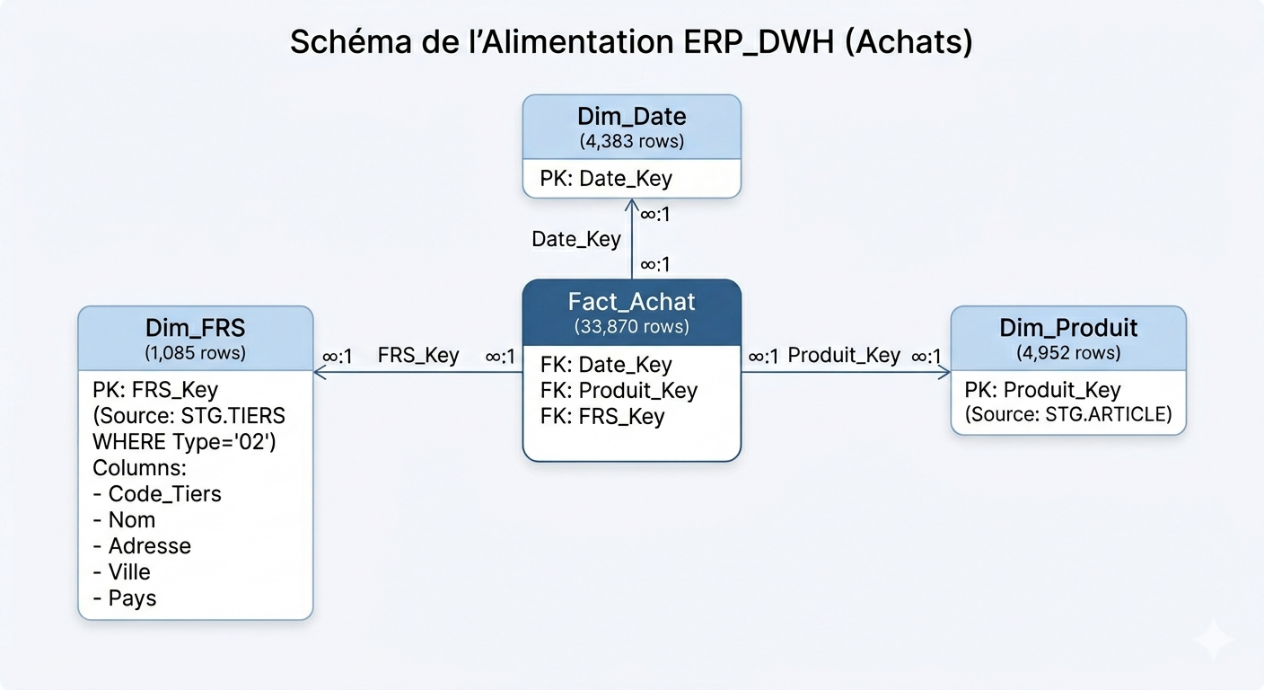
\includegraphics[width=0.7\linewidth]{Figures/Chapitre3/modele_conceptuel_achat.png}
     \caption{modèle conceptuel « Fact\_Achat »}
     \label{fig:MCachat}
 \end{figure}
\textbf{d)	Dashboarding}
\begin{itemize}
    \item \textbf{Connexion avec Power BI }
\end{itemize}
L'intégration du module Achats dans Power BI se fait en importation de deux nouvelles tables dans le modèle de données. Il s'agit de la table de faits Fact\_Achat et de la dimension Dim\_FRS. Pour bien s'intégrer à l'architecture existante et permettre des analyses croisées performantes, trois nouvelles relations ont été configurées. La table Fact\_Achat est reliée à la dimension temporelle via Fact\_Achat. Date\_Key et Dim\_Date. Date\_Key. Elle est également reliée au référentiel produit via Fact\_Achat.Produit\_Key et Dim\_Produit.Produit\_Key. Enfin, elle est reliée à son propre référentiel partenaires en connectant Fact\_Achat. FRS\_Key et Dim\_FRS. FRS\_Key.
\begin{itemize}
    \item \textbf{DAX }
\end{itemize}
La restitution visuelle de ce module se concrétise par la création d'une nouvelle vue dédiée baptisée "\textbf{Performance Achats}". Afin d'offrir une lecture immédiate de la performance aux décideurs, l'interface intègre plusieurs cartes KPI affichant le montant total des achats, le nombre de fournisseurs actifs, le coût moyen par article ainsi que la croissance des achats par rapport à l'année précédente. Ces indicateurs de haut niveau sont complétés par un ensemble de graphiques analytiques, comprenant un treemap pour la répartition des achats par fournisseur, une courbe pour suivre l'évolution temporelle des dépenses, un diagramme en barres isolant le Top 10 des fournisseurs par volume, et enfin une matrice croisant les achats par site et par famille de produits. Pour affiner l'analyse, l'utilisateur dispose de filtres contextuels basés sur la dimension temporelle (Année/Mois), le fournisseur et la catégorie de produit, tandis qu'un filtre de sécurité par site (RLS) restreint l'accès aux données selon le périmètre de l'utilisateur.\\
Pour propulser ces visuels, plusieurs mesures spécifiques ont été développées en langage DAX :
 \begin{figure}[H]
     \centering
     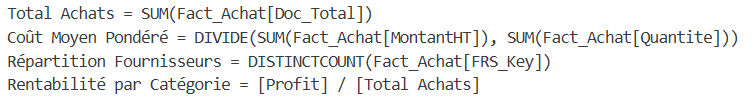
\includegraphics[width=1\linewidth]{Figures/Chapitre3/dax_achat.png}
     \caption{les DAX utilisés dans module Achat}
     \label{fig:DAXachat}
 \end{figure}
\begin{itemize}
    \item \textbf{Visuels implémentés }
\end{itemize}
 \begin{figure}[H]
     \centering
     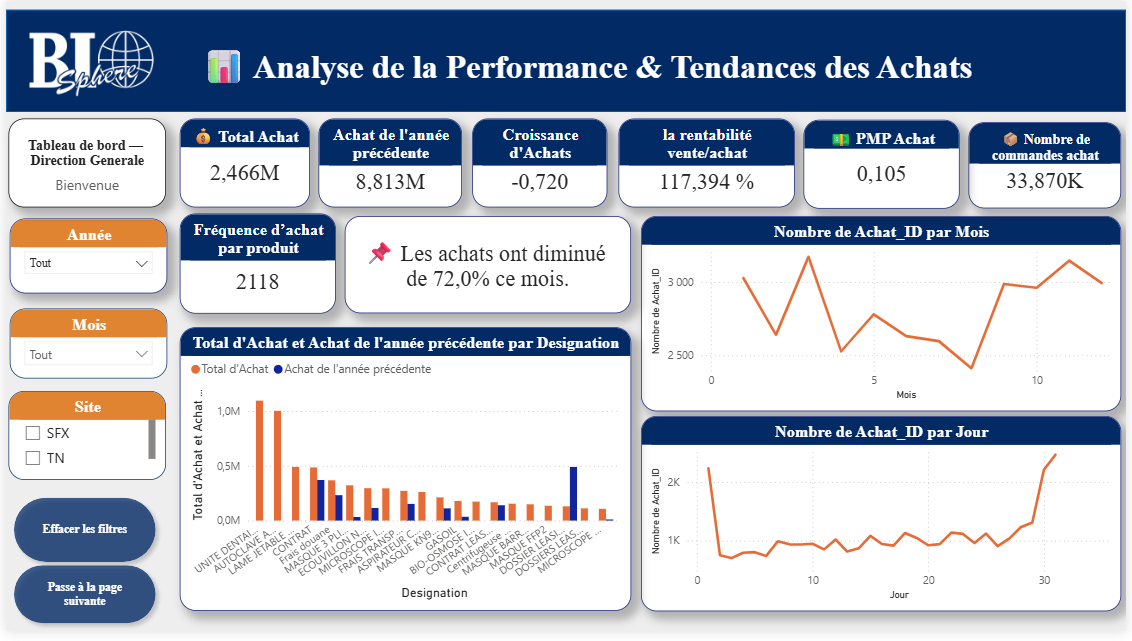
\includegraphics[width=1\linewidth]{Figures/Chapitre3/dashboard_achat.png}
     \caption{Dashboard Analyse de la performance \& tendances des achats}
     \label{fig:dashboardachat}
 \end{figure}
\subsubsection{Interprétation globale du module achats }
%================= TABLE INTERPRÉTATION MODULE ACHATS =================

{\small
\renewcommand{\arraystretch}{1.2}
\setlength{\tabcolsep}{4pt}


\begin{longtable}{|p{4.5cm}|p{4.5cm}|p{6.5cm}|}

\caption{Interprétation globale du module achats} \\

\hline
\multicolumn{1}{|c|}{\textbf{Points forts}} & 
\multicolumn{1}{c|}{\textbf{Points critiques}} & 
\multicolumn{1}{c|}{\textbf{Actions prioritaires}} \\
\hline
\endfirsthead

\hline
\rowcolor{cyan!10}
\textbf{Points forts} & \textbf{Points critiques} & \textbf{Actions prioritaires} \\
\hline
\endhead

\hline
\endfoot

Rentabilité commerciale exceptionnelle (117\%) & Chute des volumes achats (-72\% vs N-1) & Analyser les causes racines : est-ce une optimisation volontaire, un problème de trésorerie, ou des délais fournisseurs allongés ? \\
\hline

Visibilité granulaire par produit/famille & Fragmentation des commandes (33,8K transactions) & Regrouper les approvisionnements : définir des fréquences d'achat par famille pour réduire les coûts logistiques et négocier des remises volume. \\
\hline

Alerte contextuelle intégrée & Volatilité journalière \& pilotage réactif & Intégrer les prévisions IA (Sprint 3) : utiliser les modèles de classification/régression de stock pour déclencher des bons de commande anticipés plutôt que réactifs. \\
\hline

 & PMP très bas à valider par catégorie & Croiser avec le dashboard Stock : vérifier que la baisse des achats ne crée pas de ruptures sur les produits à forte rotation (LABORATOIRE, PHARMACIE). \\
\hline

\end{longtable}
}
\subsection{Sprint 3 : Module Stock}
\subsubsection{Objectifs du sprint}
Le troisième sprint a marqué une étape particulièrement complexe du projet, centrée sur la modélisation et le calcul du stock. Contrairement aux modules précédents où les indicateurs découlent de transactions directes, le stock a exigé une reconstruction complète. Le système interprète désormais la table Fact\_Stock non pas comme une photographie statique, mais comme un journal de mouvements continus. Pour obtenir une vision exacte, le stock par produit est reconstruit en cumulant l'ensemble des mouvements signés. Et pour garantir la cohérence fonctionnelle du modèle, un mécanisme de « \textit{clipping} » à zéro a été mis en œuvre pour bloquer et corriger les anomalies de stocks négatifs.
%================= TABLE SPRINT 3 =================

{\small
\renewcommand{\arraystretch}{1.2}
\setlength{\tabcolsep}{4pt}


\begin{longtable}{|p{3cm}|p{2.5cm}|p{1.6cm}|p{3cm}|p{4.5cm}|}

\caption{Sprint 3 : Module Stock} \\

\hline

\textbf{Sprint / Phase} & \textbf{User Stories concernées} & \textbf{Priorité} & \textbf{Durée estimée} & \textbf{Livrable attendu} \\
\hline
\endfirsthead

\hline
\textbf{Sprint / Phase} & \textbf{User Stories concernées} & \textbf{Priorité} & \textbf{Durée estimée} & \textbf{Livrable attendu} \\
\hline
\endhead

\hline
\endfoot

Sprint 3 : Module Stock & US04, US07, US06 & Haute & 3 semaines & Dashboard stock, alertes intelligentes \\
\hline

\end{longtable}

}
\subsubsection{Les KPIs du stock}
%================= TABLE KPIs STOCK =================

{\small
\renewcommand{\arraystretch}{1.2}
\setlength{\tabcolsep}{3pt}

\begin{longtable}{|p{2.5cm}|p{3.5cm}|p{3.5cm}|p{3.5cm}|p{3cm}|}

\caption{Les KPIs du stock} \\

\hline
\multicolumn{1}{|c|}{\textbf{Catégorie}} & 
\multicolumn{1}{c|}{\textbf{KPI}} & 
\multicolumn{1}{c|}{\textbf{Formule de calcul}} & 
\multicolumn{1}{c|}{\textbf{Source de données}} & 
\multicolumn{1}{c|}{\textbf{Fréquence}} \\
\hline
\endfirsthead

\hline
\multicolumn{1}{|c|}{\textbf{Catégorie}} & 
\multicolumn{1}{c|}{\textbf{KPI}} & 
\multicolumn{1}{c|}{\textbf{Formule de calcul}} & 
\multicolumn{1}{c|}{\textbf{Source de données}} & 
\multicolumn{1}{c|}{\textbf{Fréquence}} \\
\hline
\endhead

\hline
\endfoot

Niveau de stock & Stock total (unités) & SUM (clipped\_stock) & Fact\_Stock + reconstruction & Quotidienne \\
\hline

Disponibilité & Stock disponible & SUM(IF([Stock] > 0, [Stock], 0)) & Fact\_Stock & Quotidienne \\
\hline

Ruptures & Nombre d'articles en rupture & COUNT(IF([Stock] $\leq$ 0, 1)) & Fact\_Stock & Quotidienne \\
\hline

Valeur & Valeur totale du stock & SUM([Stock] * PUHT) & Fact\_Stock + Dim\_Produit & Mensuelle \\
\hline

Rotation & Taux de rotation des stocks & [CA] / [Stock moyen] & Fact\_Vente + Fact\_Stock & Trimestrielle \\
\hline

Performance & Taux de service & [Lignes livrées] / [Lignes commandées] * 100 & Fact\_Vente & Mensuelle \\
\hline

Alertes & Produits sous seuil critique & COUNT(IF([Stock] < [Seuil\_Min], 1)) & Fact\_Stock + Seuils & Quotidienne \\
\hline

Classification & Répartition ABC & Classification par valeur de consommation & Fact\_Stock + Fact\_Vente & Mensuelle \\
\hline

\end{longtable}

}
\subsubsection{Réalisation technique}

\textbf{a)	Extraction depuis la base BIOSPHERE}\\
La phase initiale du processus repose sur l'extraction des données de flux logistiques depuis la base source \textbf{BIOSPHERE}. Cette étape consiste à récupérer l'historique complet des flux de marchandises en interrogeant principalement la table transactionnelle \textbf{dbo.StoJou}, qui centralise l'ensemble des mouvements de stock. Pour qualifier précisément la nature de chaque transaction, une jointure est opérée avec la table \textbf{dbo.Document}, permettant ainsi d'enrichir le flux avec le type de mouvement associé. Enfin, le référentiel des articles (\textbf{dbo.Art}) est intégré au traitement afin d'associer chaque mouvement aux caractéristiques des produits correspondants.\\
Et pour garantir la pertinence et la profondeur des analyses prévisionnelles, nous avons Pris en compte exhaustive de tous les types de mouvements, à savoir \textbf{les entrées, les sorties, les retours, les transferts internes ainsi que les autres ajustements de stock.}\\

\textbf{b)	Alimentation de ERP\_STG par workflow n8n}\\
L'automatisation et la centralisation des flux logistiques au sein de la couche de staging sont opérées par le workflow n8n. Ce traitement orchestre le chargement en continu de deux tables cibles clés : STG.STOJOU, qui accueille l'ensemble des mouvements de stock bruts, et STG.CTRL\_CHARGEMENT, configurée pour assurer le suivi incrémental spécifique aux flux de stock.
 \begin{figure}[H]
     \centering
     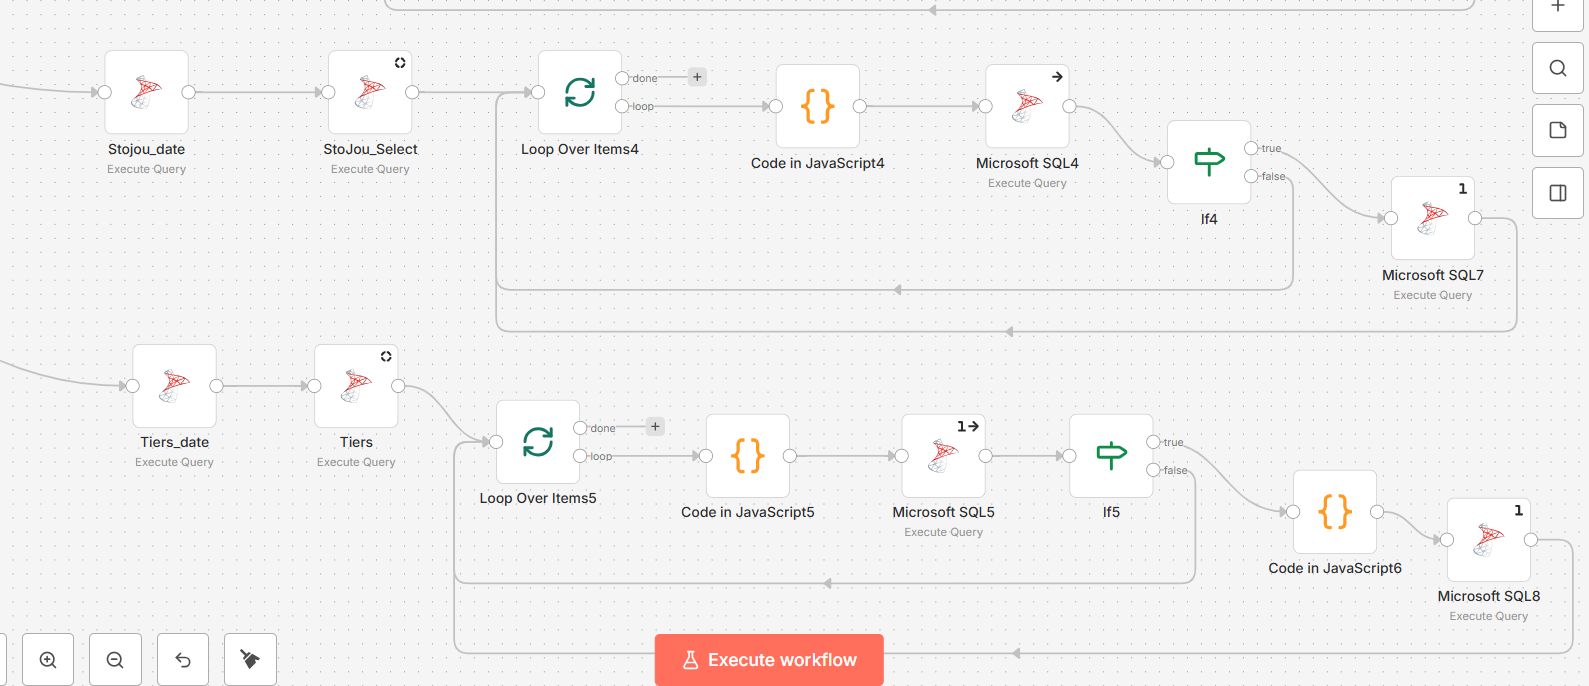
\includegraphics[width=0.99\linewidth]{Figures/Chapitre3/workflow_stock.png}
     \caption{workflow alimentation du Fact\_Stock}
     \label{fig:workflowstock}
 \end{figure}
\begin{itemize}
    \item \textbf{Transformations analytiques}
\end{itemize}
Afin de standardiser les mouvements de stock bruts et de préparer la reconstruction automatisée des volumes, les règles de classification et de valorisation algébrique suivantes sont appliquées via JavaScript :
%================= TABLE TRANSFORMATIONS ANALYTIQUES =================

{ \small
\renewcommand{\arraystretch}{1.1}
\setlength{\tabcolsep}{4.5pt}

\begin{longtable}{|p{3.2cm}|p{3.2cm}|p{2.2cm}|p{2.2cm}|}
\caption{Transformations analytiques : standardisation des mouvements de stock} \\
\hline
\multicolumn{1}{|p{3.8cm}|}{\centering\arraybackslash\textbf{Type de document (docType)}} &
\multicolumn{1}{p{3.8cm}|}{\centering\arraybackslash\textbf{Type de mouvement (stoType)}} &
\multicolumn{1}{p{2.8cm}|}{\centering\arraybackslash\textbf{Catégorie finale}} &
\multicolumn{1}{p{3cm}|}{\centering\arraybackslash\textbf{Signe mathématique}} \\
\hline
\endfirsthead

\hline
\multicolumn{1}{|p{3.8cm}|}{\centering\arraybackslash\textbf{Type de document (docType)}} &
\multicolumn{1}{p{3.8cm}|}{\centering\arraybackslash\textbf{Type de mouvement (stoType)}} &
\multicolumn{1}{p{2.8cm}|}{\centering\arraybackslash\textbf{Catégorie finale}} &
\multicolumn{1}{p{3cm}|}{\centering\arraybackslash\textbf{Signe mathématique}} \\
\hline
\endhead

\hline
\endfoot

BL (Livraison) / BV (Vente) & Tout type & SORTIE & -1 \\
\hline

BF (Fabrication) / FA (Achat) & Tout type & ENTREE & +1 \\
\hline

RET (Retour) & Tout type & RETOUR & +1 \\
\hline

Tout type & TRANSFER & INTERNE & 0 \\
\hline

Autres configurations & Autres configurations & AUTRE & 0 \\
\hline

\end{longtable}

}
Le script JavaScript applique deux règles essentielles pour standardiser les mouvements de stock. D'abord, il classifie chaque transaction selon son origine : les ventes et livraisons deviennent des Sorties, les achats et fabrications des Entrées, les retours restent des Retours, et les transferts sont classés comme Internes. Ensuite, il attribue un signe mathématique à chaque catégorie pour permettre le calcul automatique des volumes : un signe positif (+1) augmente le stock (entrées et retours), un signe négatif (-1) le diminue (sorties), et un signe neutre (0) est appliqué aux mouvements internes ou indéterminés pour éviter d'en fausser le calcul global.\\

\textbf{c)	Alimentation de ERP\_DWH}\\
L'intégration des flux logistiques dans la couche décisionnelle aboutit à la création de la table de faits centrale appelée Fact\_Stock. Cette table contient 371 512 lignes. La structure de cette table est configurée de manière à suivre le niveau de stock global. 
 \begin{figure}[H]
     \centering
     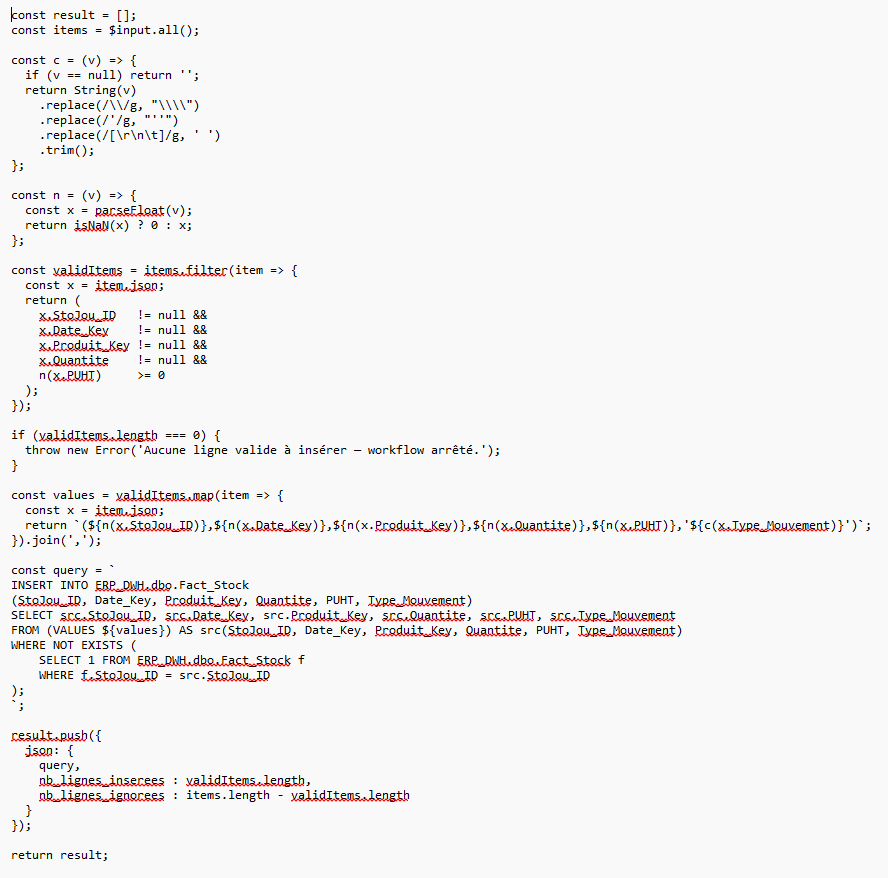
\includegraphics[width=0.8\linewidth]{Figures/Chapitre3/code_js_stock.png}
     \caption{Exemple du code JS pour insertion de la table stg.stock}
     \label{fig:codeJSstock}
 \end{figure}
 \begin{figure}[H]
     \centering
     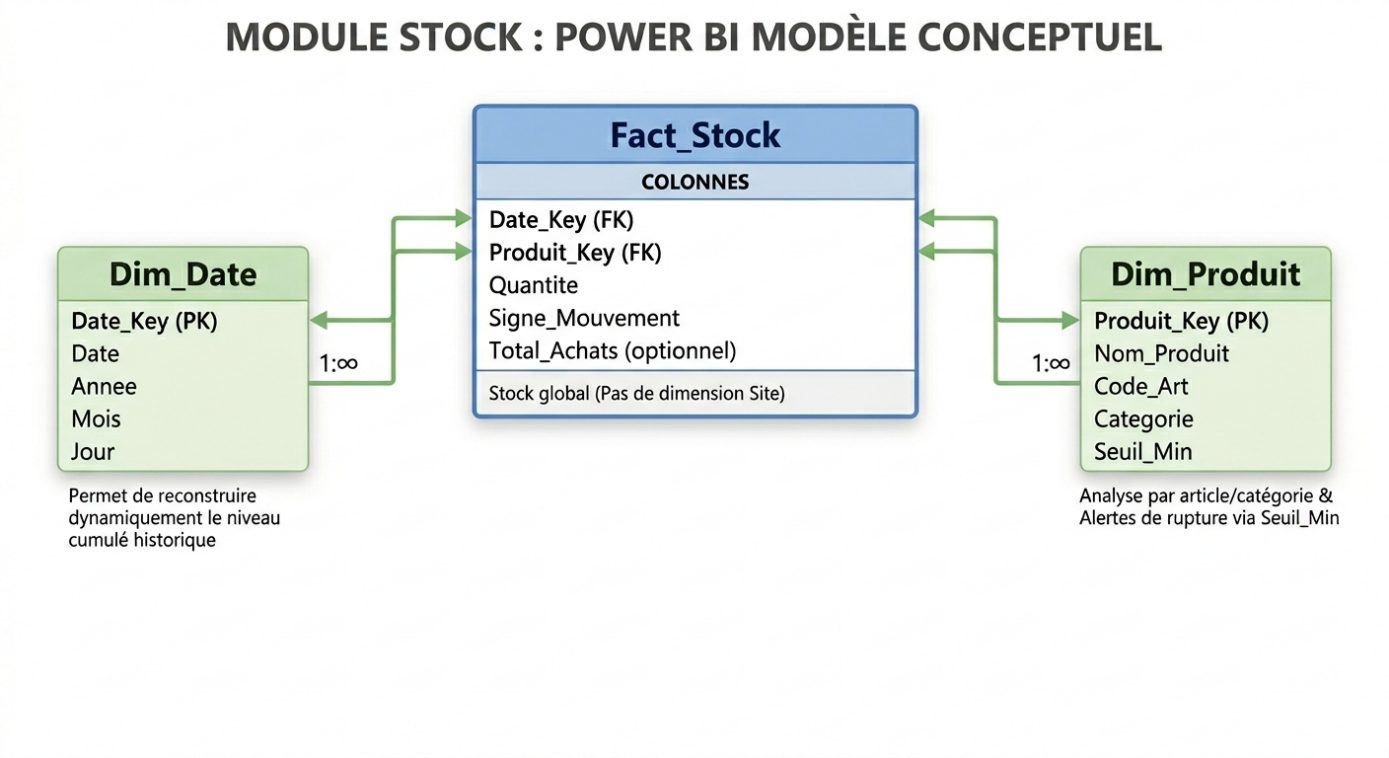
\includegraphics[width=0.8\linewidth]{Figures/Chapitre3/modele_conceptuel_stock.png}
     \caption{modèle conceptuel « Fact\_Stock »}
     \label{fig:MCstock}
 \end{figure}
\textbf{d)	Dashboarding}\\
L'intégration des données de stock dans l'environnement Power BI s'effectue par l'importation de la table de faits Fact\_Stock. Et pour garantir la cohérence des analyses transversales, cette table est connectée aux dimensions communes du Galaxy existante via deux relations de type un-à-plusieurs (1:$\infty$) d'une part, Fact\_Stock.Date\_Key pointe vers Dim\_Date.Date\_Key et, d'autre part, Fact\_Stock.Produit\_Key est reliée à Dim\_Produit.Produit\_Key.
\begin{itemize}
    \item \textbf{DAX}
\end{itemize}
Pour modéliser le comportement du stock et suivre la santé logistique des articles, les mesures DAX suivantes ont été développées :
 \begin{figure}[H]
     \centering
     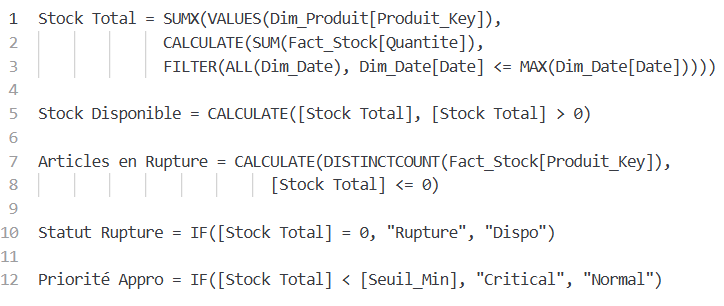
\includegraphics[width=0.9\linewidth]{Figures/Chapitre3/dax_stock.png}
     \caption{exemple des DAX du dashboard Analyse du stock \& inventory health}
     \label{fig:DAXstock}
 \end{figure}
\begin{figure}[H]
    \centering
    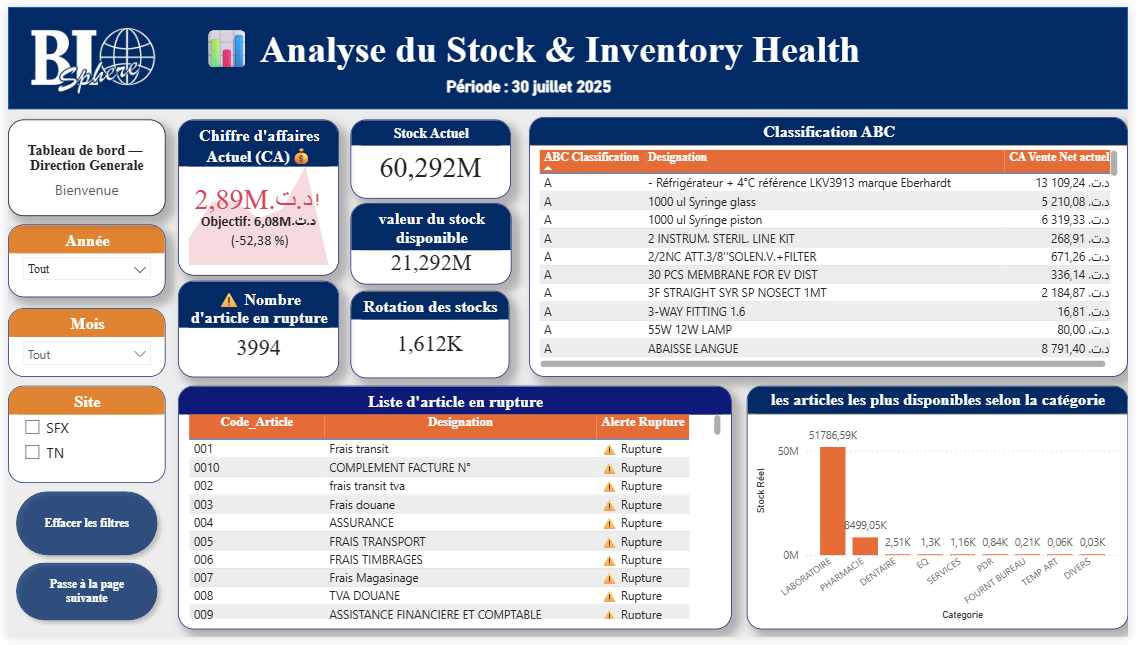
\includegraphics[width=1\linewidth]{Figures/Chapitre3/dashboard_stock.png}
    \caption{Dashboard Analyse du stock \& inventory health}
    \label{fig:placeholder}
\end{figure}
\subsubsection{Interprétation globale du module stock}
%================= TABLE INTERPRÉTATION MODULE STOCK =================

{\small
\renewcommand{\arraystretch}{1.2}
\setlength{\tabcolsep}{4pt}


\begin{longtable}{|p{4.5cm}|p{4.5cm}|p{7cm}|}

\caption{Interprétation globale du module stock} \\

\hline
\multicolumn{1}{|c|}{\textbf{Points forts}} & 
\multicolumn{1}{c|}{\textbf{Points critiques}} & 
\multicolumn{1}{c|}{\textbf{Actions prioritaires}} \\
\hline
\endfirsthead

\hline
\rowcolor{cyan!20}
\textbf{Points forts} & \textbf{Points critiques} & \textbf{Actions prioritaires} \\
\hline
\endhead

\hline
\endfoot

Visibilité granulaire sur les ruptures \& classification ABC & Nombre d'articles en rupture très élevé (3 994) & Filtrer les ruptures ``métier'' : exclure les postes administratifs/comptables pour obtenir un indicateur logistique fiable. \\
\hline

Suivi de la rotation et valorisation du stock & Écart important Stock Actuel vs Stock Disponible & Auditer les stocks bloqués : identifier la nature des 39M TND non disponibles et accélérer leur remise en circulation ou leur écriture. \\
\hline

Interface claire avec filtres Année/Mois/Site & CA à -52\% de l'objectif & Croiser ruptures \& ventes : vérifier si les ruptures impactent directement le chiffre d'affaires et prioriser les réapprovisionnements sur les articles A. \\
\hline

 & Concentration forte sur Laboratoire & Intégrer les prévisions IA : utiliser les modèles de classification/régression pour anticiper les ruptures et déclencher des alertes avant l'impact commercial. \\
\hline

\end{longtable}
}

\section{Conclusion}
Ce chapitre a permis de présenter la mise en œuvre technique du système décisionnel à travers la conception du Data Warehouse, l’automatisation des processus ETL et le développement des tableaux de bord analytiques sécurisés. Les différentes problématiques rencontrées, principalement le niveau de la gestion et de l’interprétation des stocks qui ont mis en évidence la nécessité d’intégrer une approche prédictive capable d’anticiper les risques de rupture et les variations futures. Ainsi, la réalisation du Sprint 4 consacré à l’intelligence artificielle et à la prévision des stocks devient une étape essentielle pour faire évoluer le système vers une aide à la décision proactive et intelligente. 



